\section{System Architecture}
\label{sec:architecture}

\subsection{Quality Attributes}
\label{sec:architecture-quality}

Quality attributes are defined in order to ensure the architectural
decisions made when creating the system architecture not only provide
the required functionality, but also produce a system meeting the
expectations of all stakeholders. For example the system may be
expected to meet certain security standards or availability
levels. Explicitly defining these quality attributes before concretely
designing a system allows for the correct tactics and patterns to be
adopted in order to maximise the utility of important qualities.

When examining the HUMS non-functional requirements the following
system quality attributes were identified:

\begin{center}
  \textit{Availability, Performance, Modifiability, Security,
    Testability, Usability}
\end{center}

Of these, availability, performance, security and usability can be
observed and measured, the others are unobservable though steps can
still be taken to maximise their utility.  Of these availability,
performance, security and usability can be observed and measured, the
others are unobservable however steps can still be taken to maximise
their utility. For the prototype implementation, at this stage,
usability and security have not been heavily considered, however in
the real system they would be of high importance.

%Maybe go into more detail if space

Availability defines how ready the system is to be used, and is
normally the percentage of downtime over a specified timeframe. The
desired utility of the quality attribute within the HUMS, as defined
by the non-functional requirements, is 99.9\% per month. Since lack of
availability is often linked to faults occurring, fault detection and
recovery tactics (such as the use of runtime exceptions, redundancy
through backups and transactions) could be employed in order to
achieve the desired level of availability.

The performance of a system is normally measured by its latency and
throughput. The HUMS is required to dispatch notifications through the
notification generator after events have been triggered by the
analysis controller, with a latency less than 5ms, the system is also
required to be able to support multiple data output clients. Tactics
such as reducing overhead though careful use of data structures and
prioritising events can help reduce latency, at least for the most
important events, defined by the end user. It may also be possible to
add concurrency, such that multiple notification threads are used when
demand for notifications and reports are high, reducing the bottleneck
created at the notification generator.

Modifiability is one of the most important qualities of the HUMS,
though not measurable, lack of modifiability can increase the cost and
time taken to complete the project. The HUMS will initially be built
to tackle a single domain (software), however will in the future be
required to work on embedded systems, mechanical systems, electrical
systems and even people. In order to ensure these changes are as
efficient as possible the initial system must be modifiable. Tactics
that can be used to increase the modifiability of the system include
using small modules within the system, decreasing the coupling between
those modules and increasing the cohesion. In order to achieve low
coupling the HUMS uses interfaces between modules and restricts
dependencies, such that the majority of modules can be swapped out
without large changes to the overall system.

\subsection{System Views}
\label{sec:architecture-views}

When designing the HUMS we identified four different views of of the
system which must be documented:

\begin{description}
  \item[Module View] The required software modules and relationships
    between them at a high level.

  \item[Behavioural View] The flow of data and dynamic actions within
    the system.

  \item[Deployment View] How modules are geographically positioned.

  \item[Conceptual View] Class diagrams, showing a concrete
    implementation of the functionality.
\end{description}

\subsection{Module View}
\label{sec:architecture-moduleview}

Having determined the quality attributes of the HUMS and the tactics
which can be employed in order to achieve a high utility of these
qualities, a conceptual view can be formed. The conceptual diagram
shown in figure \ref{fig:moduleDiagram} depicts the modules of the
HUMS and the interactions between these modules at a high level.

%%TODO this diagram doesn't show the core or have a key

\begin{figure}[ht!]
  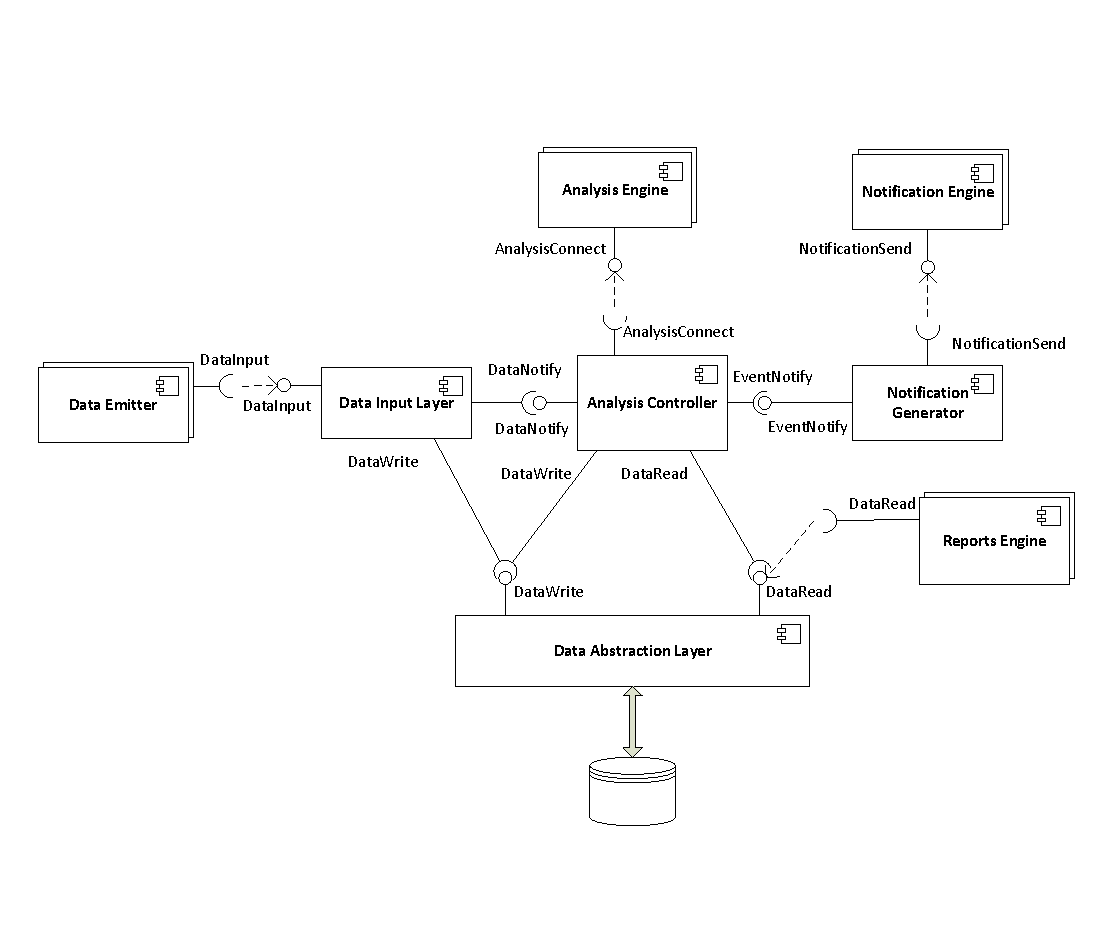
\includegraphics[width=13cm]{images/moduleDiagram.pdf}
  \caption{The module diagram of the HUMS}
  \label{fig:moduleDiagram}
\end{figure}

\begin{description}
  \item[Data Emitter] Sends data to the system core in a standard
    format. May be included within the HUMS or created by the end
    user.

  \item[Data Input Layer] Receives data from a data emitter and sends
    it to the data abstraction layer. Alerts the analysis controller
    that new data was received.

  \item[Data Abstraction Layer] Handles all interaction with the
    database, such that if the database was to be altered, only this
    layer would need to change.

  \item[Analysis Controller] Alert the analysis engines when new data
    has arrived, pulling the required data from the data abstraction
    layer. If an analysis engine determines an event has occurred
    within the data then the analysis controller forwards that event
    to the notification generator.

  \item[Analysis Engine] Analyses the data looking for trends, if a
    trend is found an event is returned to the analysis
    controller. Analysis engines may be included in the HUMS or
    created by the end user.

  \item[Notification Generator] Receives events from the analysis
    controller, defines an abstract notification and sends it to the
    appropriate notification engine.

  \item[Notification Engine] Receives an abstract notification from
    the notification generator and creates a concrete notification,
    for example an email or triggering a change in system
    behaviour. Notification engines may be included in the HUMS or
    created by the end user.

  \item[Reports Engine] Pulls data from the data abstraction layer and
    formats it into a report, for example a PDF or graph. Reports
    engines may be included in the HUMS or created by the end user.
\end{description}

\subsection{Behavioural View}
\label{sec:architecture-behaviouralview}

The module view shows how modules of the system are connected, however
does not fully represent the interactions between components and the
dynamic actions of the system. A behavioural view can be used to
detail this information, showing the flow of data and events within
the HUMS. Figure \hl{XXX} shows the behavioural model of the HUMS,
detailing how the HUMS goes from receiving data from a data emitter to
generating a notification.

%%Input Diagram WITH KEY

\subsection{Deployment View}
\label{sec:architecture-deploymentview}

With view to deployment the HUMS needs to be tailorable, the core
system may be running on the same hardware as the data emitter, it may
also be geographically distant. Engines may all be on separate
machines or may all be together. Figures \hl{XXX and XXX} show the
main scenarios for deployment of the HUMS, with a view that if the
system architecture can perform under these situations, then it can
perform under all others.

\hl{We also chose to look at deploying the system as a service....}

%% TODO talk about admin centre shizzle

\subsection{Conceptual View}
\label{sec:architecture-conceptualview}

\subsubsection{Data Input Layer}
\label{sec:architecture-conceptualview-input}

The data input layer, shown in figure \ref{fig:dataInputLayer},
contains the following classes:

\begin{description}
  \item[DataInputServer] An object which starts up a multithreaded
    server to receive connections, and which periodically processes
    received data by sending it off to the database and notifying the
    analysis component. It accesses these by having references to them
    passed in upon creation.

  \item[ProtoReceiver] Listens on a socket for inbound connections,
    and then hands them off to a new ProtoMultiReceiver, running in a
    new thread, for processing. It also maintains a thread-safe
    concurrent queue, which all of the receivers write to, and the
    server reads (and removes) from. This use of multithreading
    enables multiple clients to send data at the same time easily, and
    the use of a queue ensures that data is inserted into the database
    in the order in which it is received.

  \item[ProtoMultiReceiver] Receives data from a particular data input
    client, writing received data to the queue.
\end{description}

\begin{figure}[ht!]
  \centering
  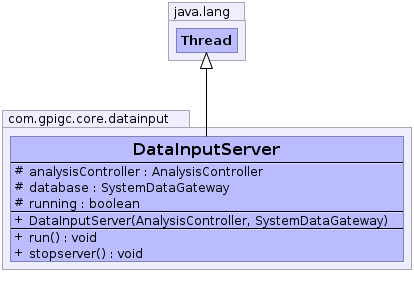
\includegraphics[width=7cm]{images/DataInputLayer/DataInputServer.png}
  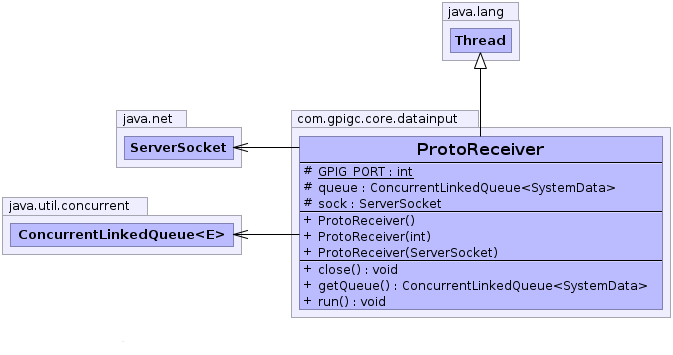
\includegraphics[width=12cm]{images/DataInputLayer/ProtoReceiver.png}
  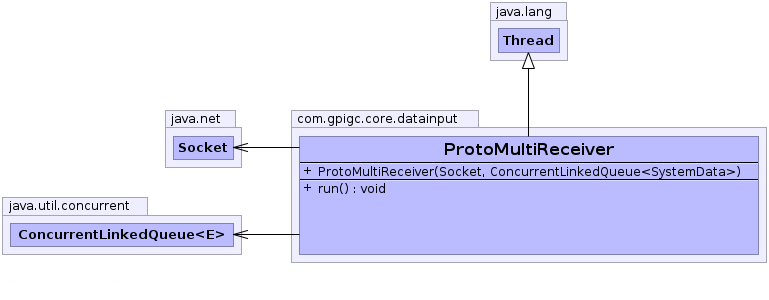
\includegraphics[width=12cm]{images/DataInputLayer/ProtoMultiReceiver.png}
  \caption{Conceptual diagrams of the data input layer classes, using UML 2 notation}
  \label{fig:dataInputLayer}
\end{figure}

\subsubsection{Data Abstraction Layer}
\label{sec:architecture-conceptulview-abstraction}

The data abstraction layer, shown in figure
\ref{fig:dataAbstractionPackage}, contains the following classes:

\begin{description}
  \item [System Data Gateway] An interface used to abstract the
    datastore implementation details from the rest of the
    application. An implementation of this interface will provide ways
    to read and write from the chosen datastore, meaning the rest of the
    system is not concerned with the datastore implementation. When
    interfacing with a datastore the end user will be required to
    implement this interface.

  \item [EmitterSystemState] An object representing the data received
    from a data emitter at a particular time. The state object holds
    the ID of the end user's system and the creation timestamp along
    with a map of sensor IDs against the value of the sensor at that
    particular time. A map was used to represent the sensors and
    values so that the end user is free the send data from as many or
    as few sensors at a time, reducing the number of writes to the
    database. For serialisation this object includes methods to
    convert to and from JSON.

  \item [DataJSONAttribute] An enumeration that wraps up the keys used
    to look up values in the JSON serialisations of the
    EmitterSystemState and QueryResult classes.

  \item [SensorState] An object representing the state of a particular
    system sensor. A sensor has an ID, a value and two timestamps, one
    specifying the time the sensor value was added to the database and
    the other the time the value was created.

  \item [QueryResult] An object representing the result of a database
    query, containing the ID of the end user's system to which the
    data relates and a list of sensor states pulled from the database.
\end{description}

\begin{figure}[ht!]
  \centering
  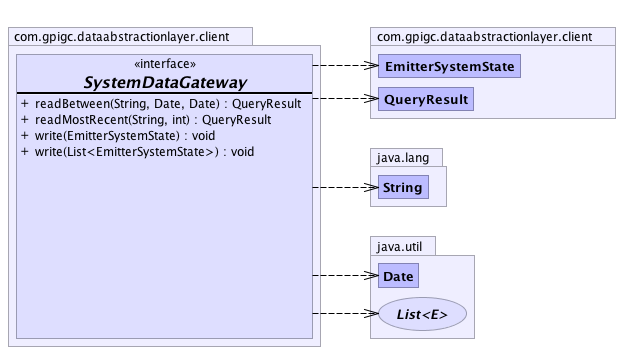
\includegraphics[width= 9.5cm]{images/DataAbstractionLayer/systemDataGateway.png}
  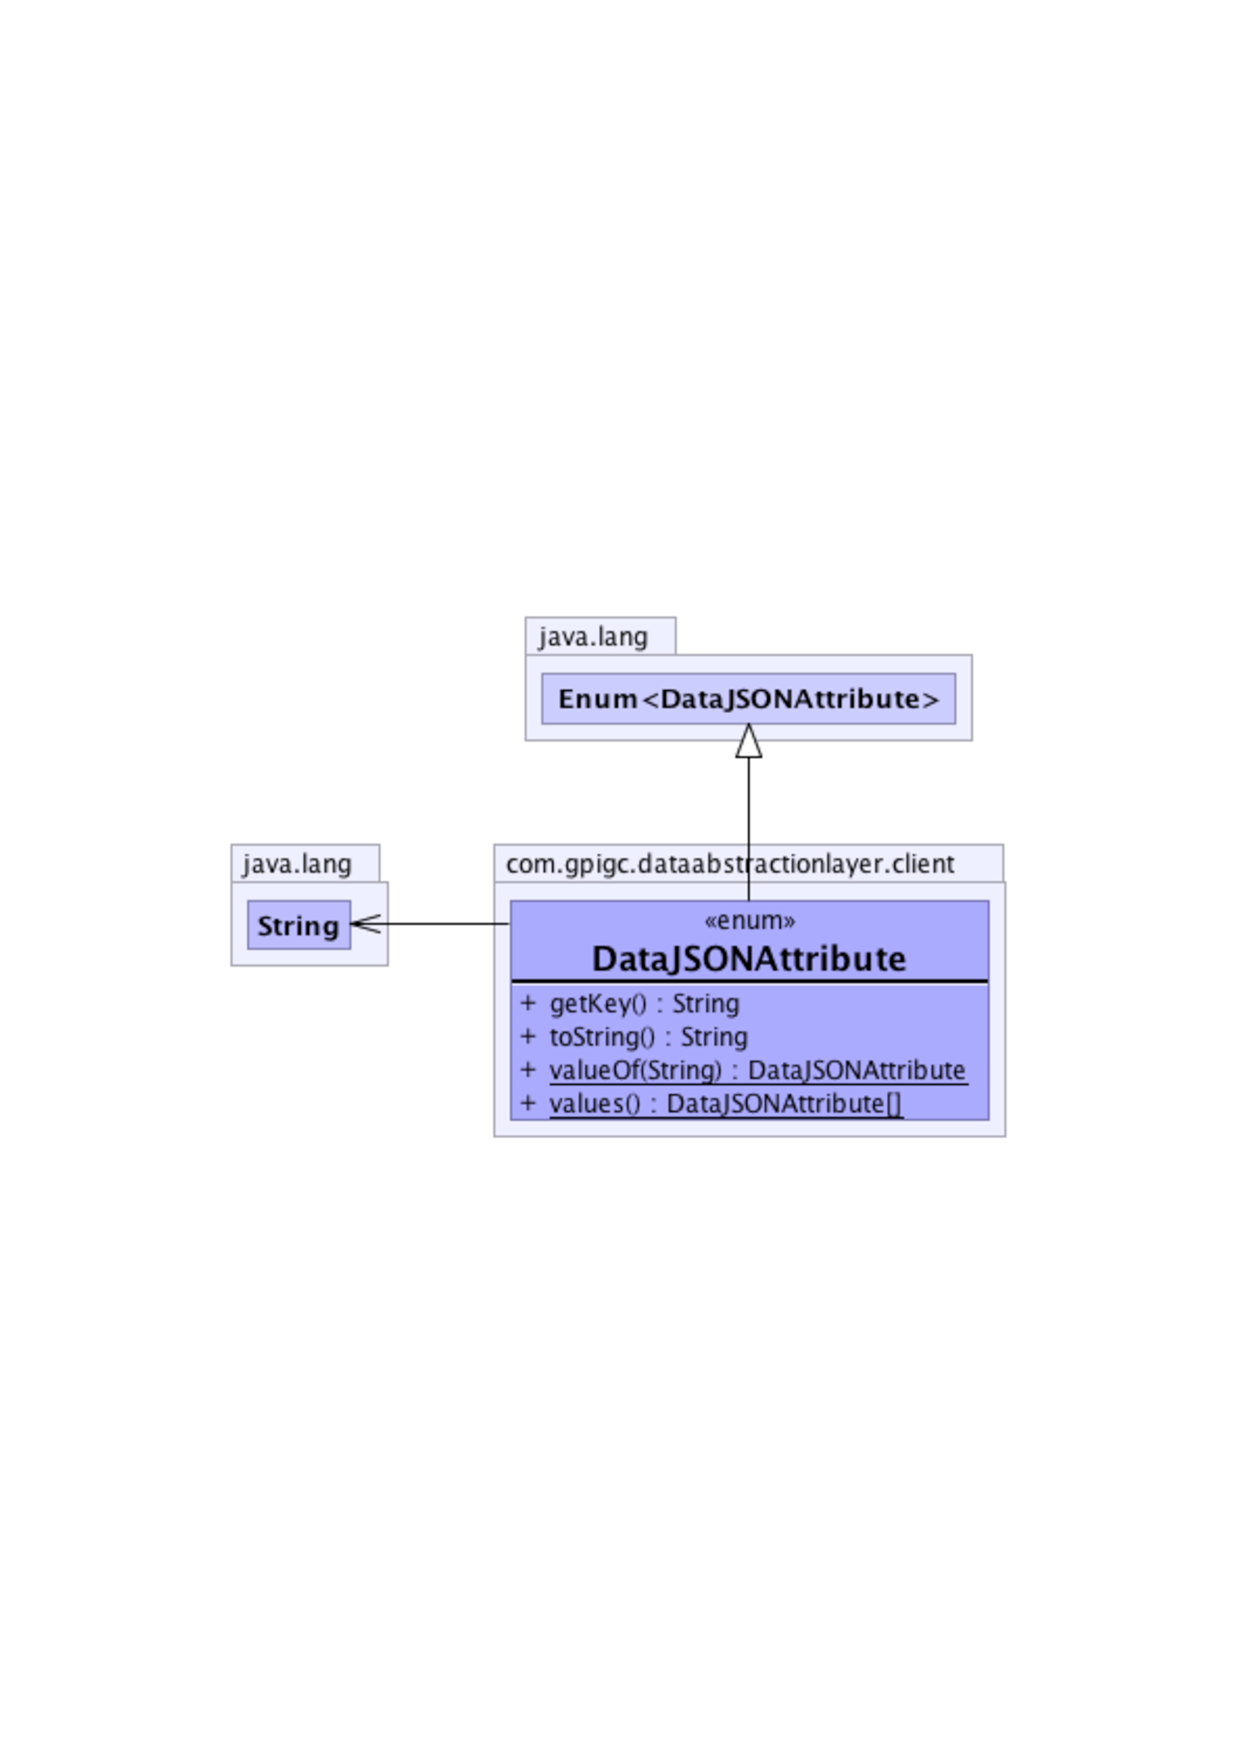
\includegraphics[width= 5cm]{images/DataAbstractionLayer/dataJsonAttribute.pdf}
  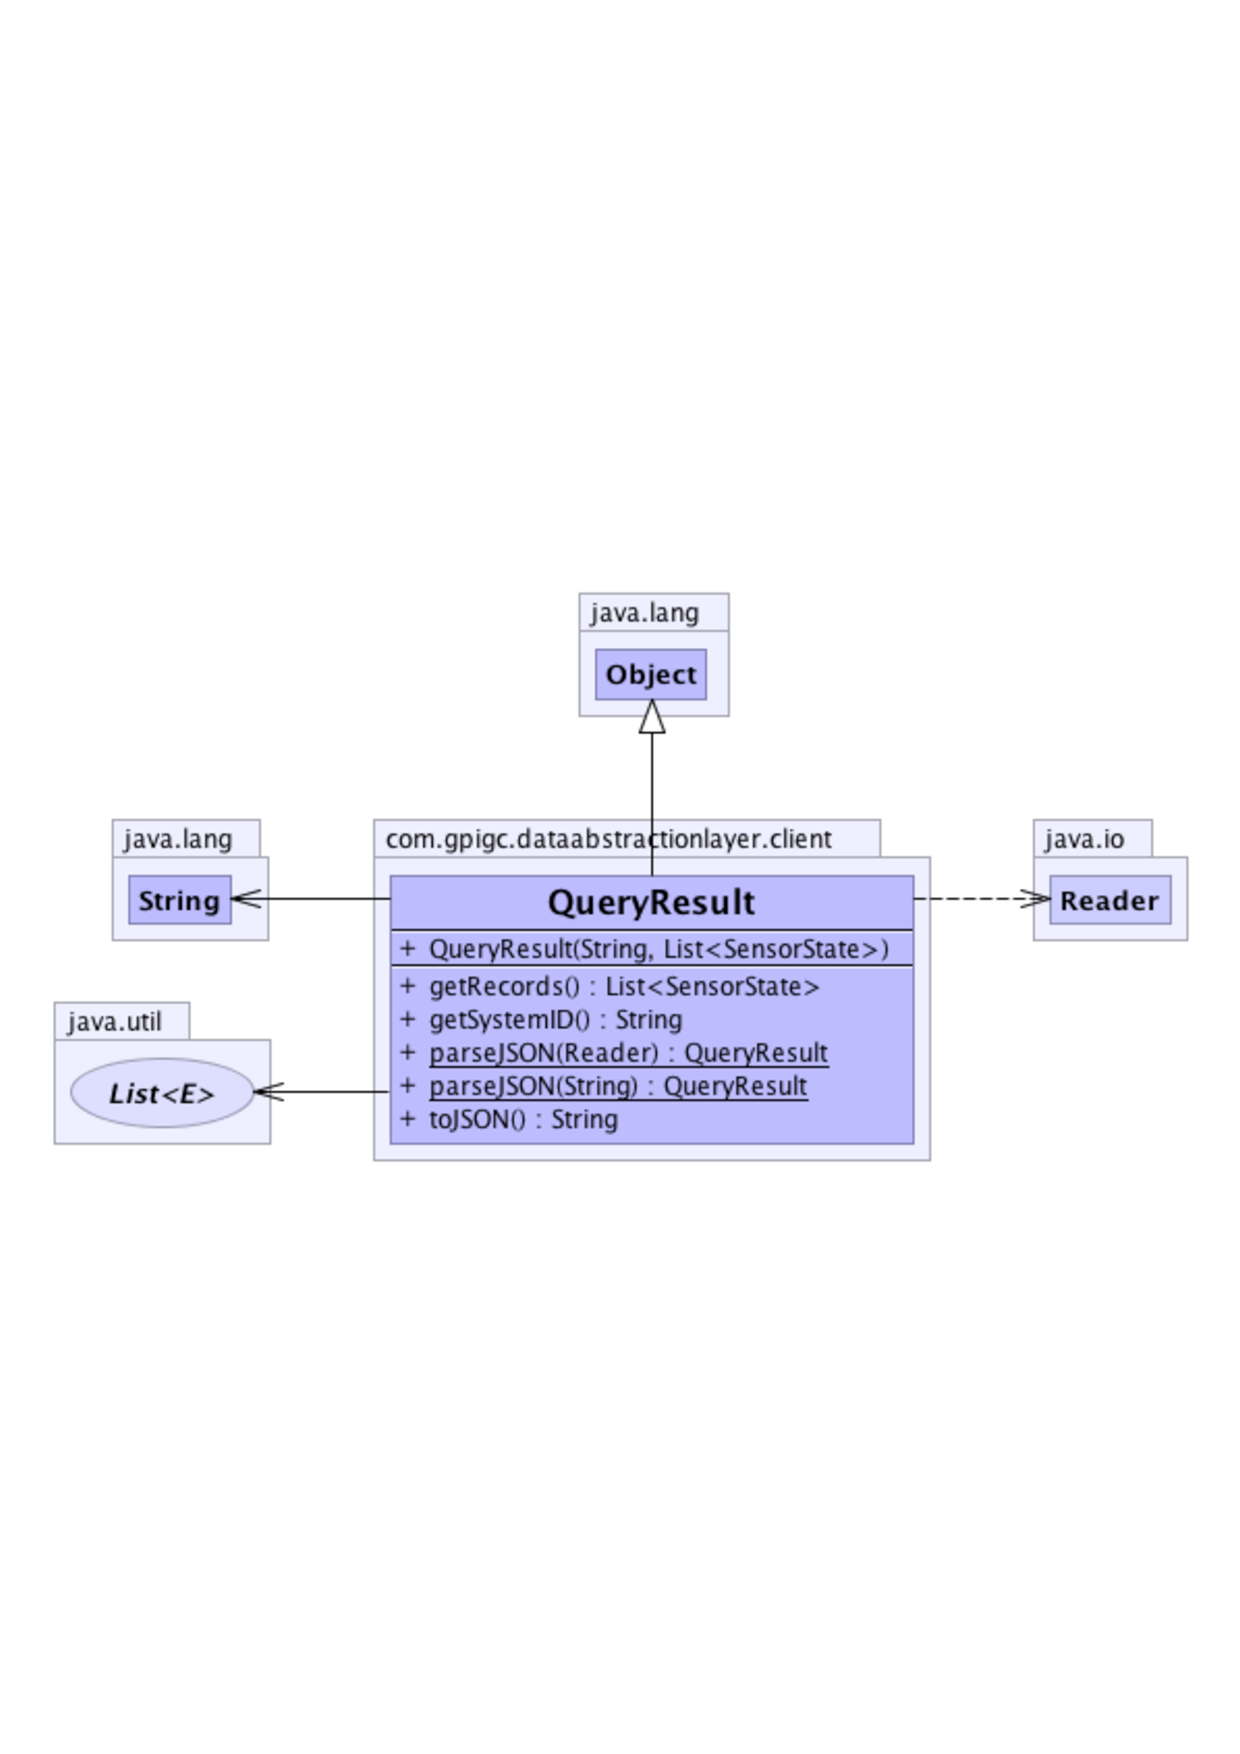
\includegraphics[width= 7cm]{images/DataAbstractionLayer/queryResult.pdf}
  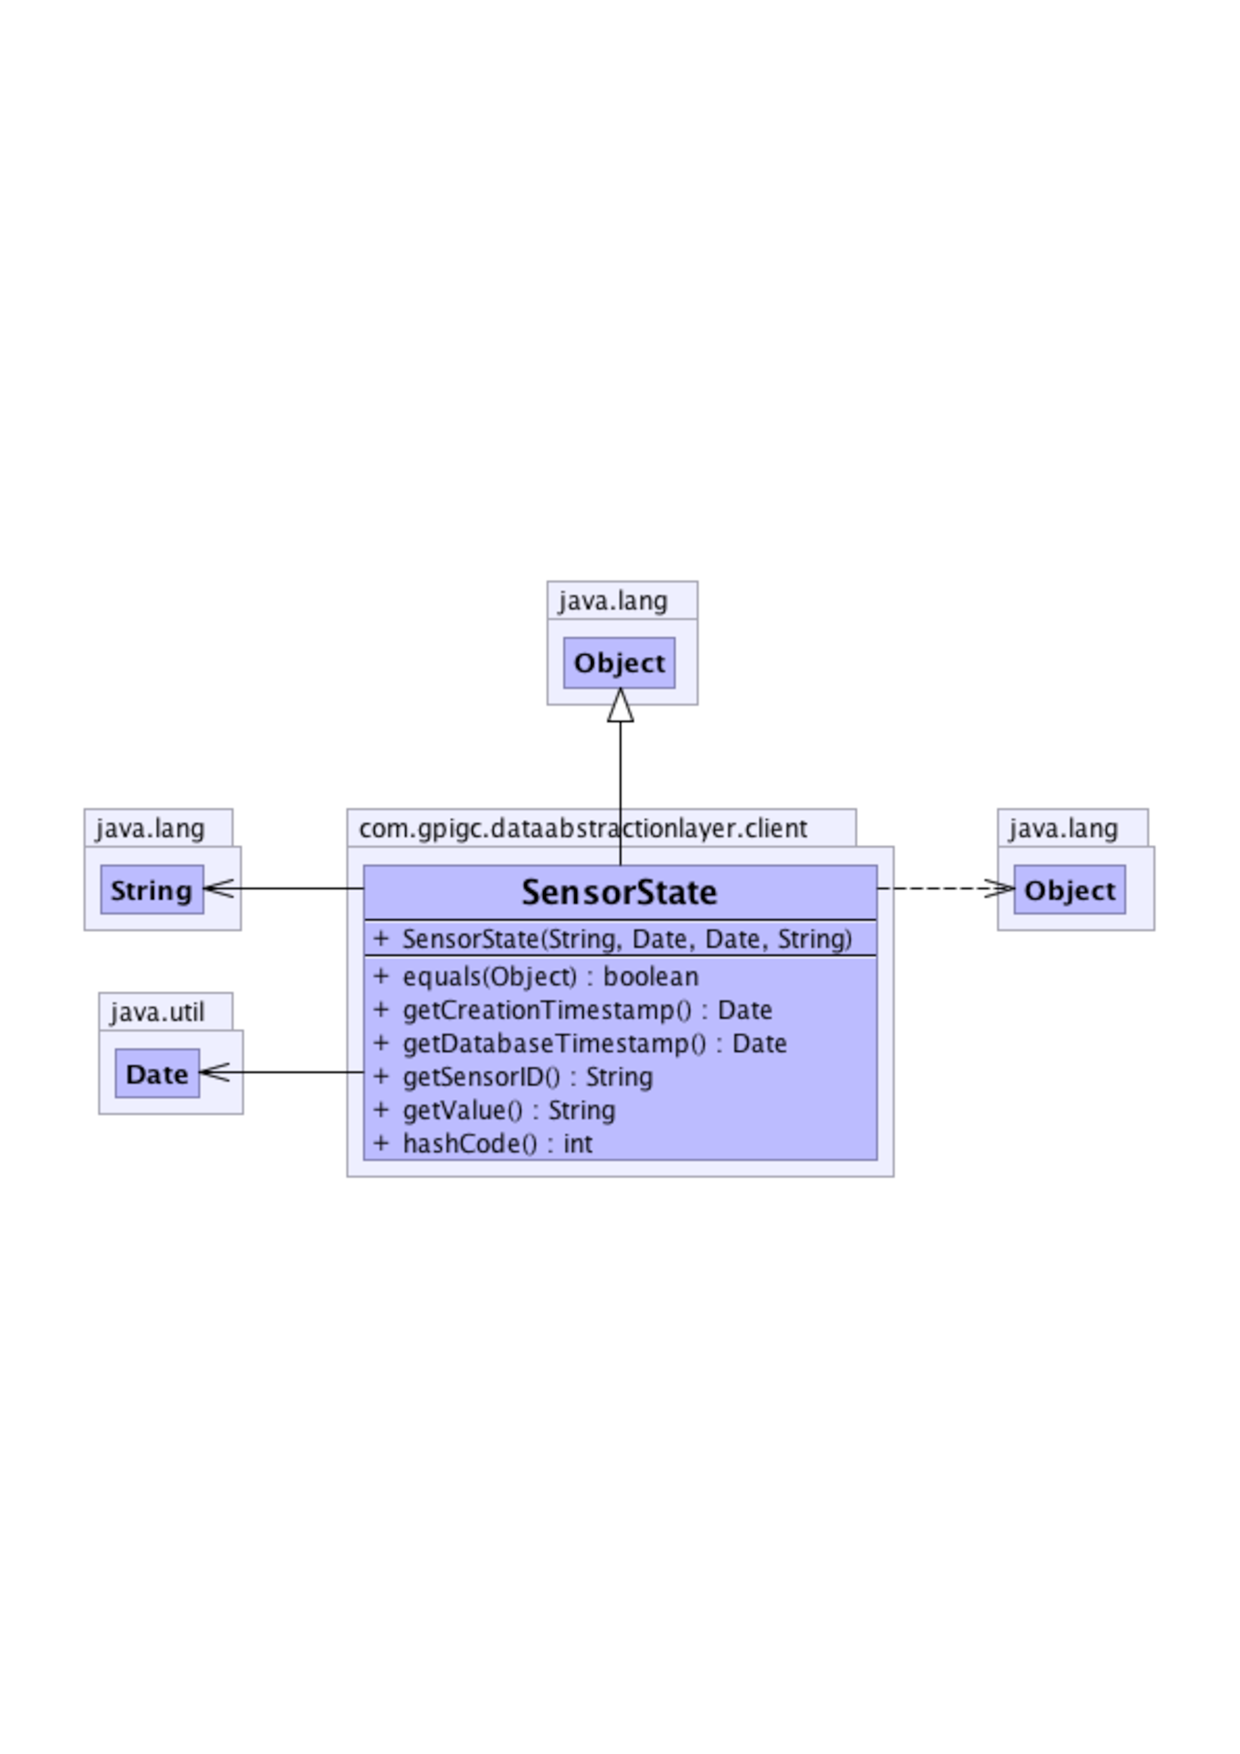
\includegraphics[width= 7cm]{images/DataAbstractionLayer/sensorState.pdf}
  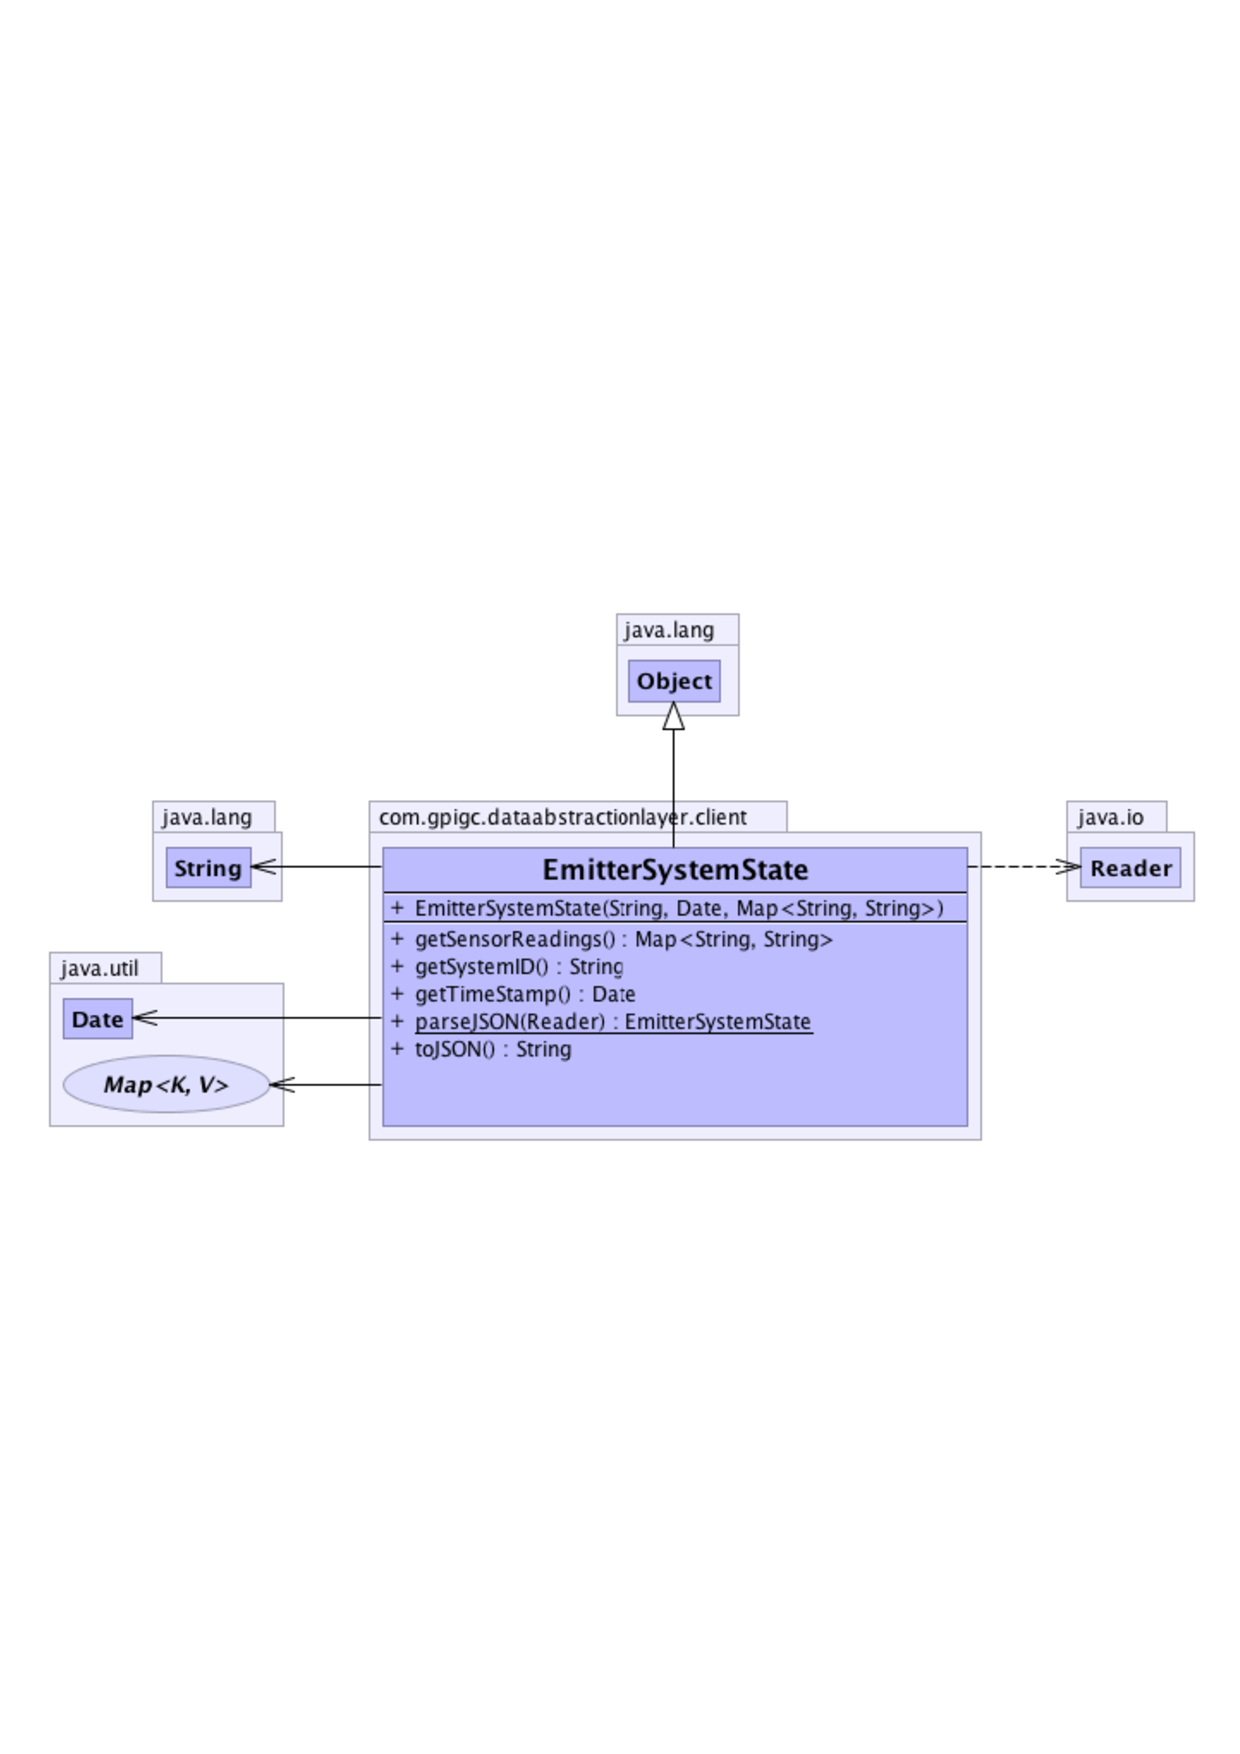
\includegraphics[width= 9cm]{images/DataAbstractionLayer/emitterSystemState.pdf}
  \caption{Conceptual diagrams of the data abstraction layer classes, using UML 2 notation}
  \label{fig:dataAbstractionPackage}
\end{figure}

\subsubsection{Analysis Component}
\label{sec:architecture-conceptualview-analysis}

The analysis component, shown in figure
\ref{fig:dataAnalysisComponent}, contains the following classes:

\begin{description}
  \item [Analysis Controller] An object that coordinates all analysis of
    sensor data. The object interfaces with the data input layer,
    receiving a system ID when analysis is required. Once analysis has
    been carried out the controller processes the results and triggers
    notifications where appropriate. Analysis engines are associated
    with the analysis controller by class loading allowing for users to
    add and remove analysis engines at run-time.

  \item [Analysis Engine] An abstract class that implements the basic
    functionality and defines the methods required of an implemented
    analysis engine. Each engine has a list of associated systems. The
    implementation of the analyse method interfaces with database
    abstraction layer to retrieve the appropriate sensor data and then
    performs the desired analysis. Once analysis is complete the engine 
    returns a result object. When creating their own analysis 
    engines the end user will be required to extend this class, implement 
    the abstract methods and define what constitutes an event.

  \item [Mean Analysis] An object that extends the analysis engine
    class and implements mean analysis. When called by the analysis
    controller, sensor data is retrieved for all associated systems
    and mean analysis is performed. If any mean values fall outside of
    the acceptable bounds then a notification is raised.

  \item [Result] An object representing the result of the analysis
    carried out by the chosen analysis engine. The object contains a
    map of any data to be saved back to the database and a flag
    indicating whether a notification needs to be triggered. For
    serialisation the data to be saved to the database is stored in a
    map of string key-values. When implementing their own analysis
    engine the end user will be able to specify what data is to be
    saved back to the database.

  \item [Event Notify] An object representing a notification,
    containing the name of the analysis engine that triggered the
    notification, the ID of the system that the notification applies
    to and the result object from the analysis engine that triggered
    the notification.
\end{description}

\begin{figure}[ht!]
  \centering
  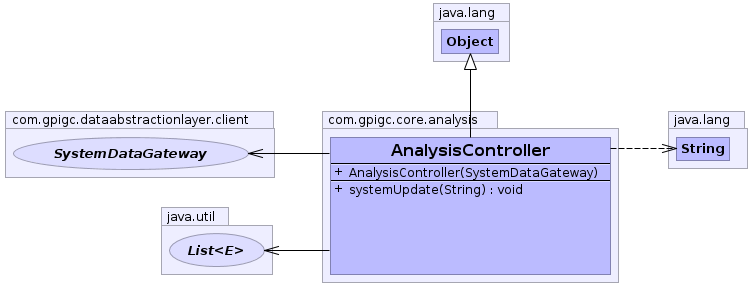
\includegraphics[width= 9.5cm]{images/Analysis/AnalysisController.png}
  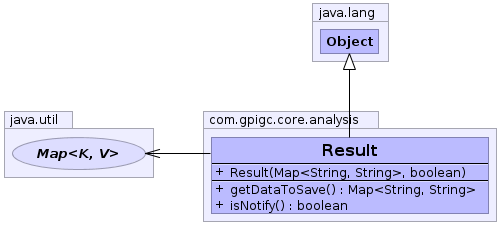
\includegraphics[width= 5cm]{images/Analysis/Result.png}
  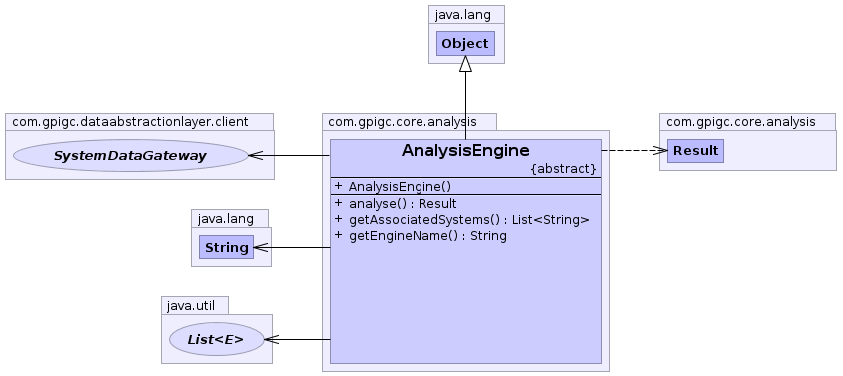
\includegraphics[width= 12cm]{images/Analysis/AnalysisEngine.png}
  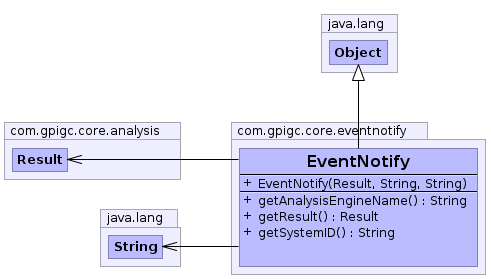
\includegraphics[width= 6cm]{images/Analysis/EventNotify.png}
  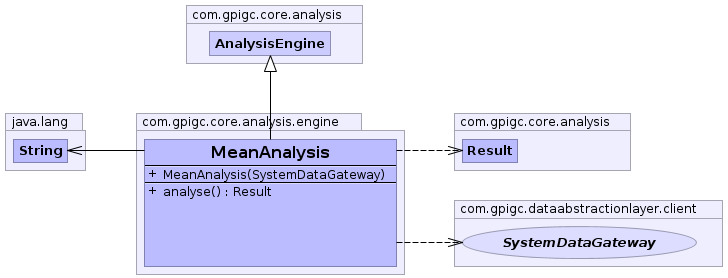
\includegraphics[width= 8cm]{images/Analysis/MeanAnalysis.png}
  \caption{Conceptual diagrams of the analysis component classes, using UML 2 notation}
  \label{fig:dataAnalysisComponent}
\end{figure}

\subsubsection{Notification Generator}
\label{sec:architecture-conceptualview-notification}

%%Class diagrams WITH KEYS
